\documentclass[twoside]{book}

% Packages required by doxygen
\usepackage{fixltx2e}
\usepackage{calc}
\usepackage{doxygen}
\usepackage[export]{adjustbox} % also loads graphicx
\usepackage{graphicx}
\usepackage[utf8]{inputenc}
\usepackage{makeidx}
\usepackage{multicol}
\usepackage{multirow}
\PassOptionsToPackage{warn}{textcomp}
\usepackage{textcomp}
\usepackage[nointegrals]{wasysym}
\usepackage[table]{xcolor}

% Font selection
\usepackage[T1]{fontenc}
\usepackage[scaled=.90]{helvet}
\usepackage{courier}
\usepackage{amssymb}
\usepackage{sectsty}
\renewcommand{\familydefault}{\sfdefault}
\allsectionsfont{%
  \fontseries{bc}\selectfont%
  \color{darkgray}%
}
\renewcommand{\DoxyLabelFont}{%
  \fontseries{bc}\selectfont%
  \color{darkgray}%
}
\newcommand{\+}{\discretionary{\mbox{\scriptsize$\hookleftarrow$}}{}{}}

% Page & text layout
\usepackage{geometry}
\geometry{%
  a4paper,%
  top=2.5cm,%
  bottom=2.5cm,%
  left=2.5cm,%
  right=2.5cm%
}
\tolerance=750
\hfuzz=15pt
\hbadness=750
\setlength{\emergencystretch}{15pt}
\setlength{\parindent}{0cm}
\setlength{\parskip}{3ex plus 2ex minus 2ex}
\makeatletter
\renewcommand{\paragraph}{%
  \@startsection{paragraph}{4}{0ex}{-1.0ex}{1.0ex}{%
    \normalfont\normalsize\bfseries\SS@parafont%
  }%
}
\renewcommand{\subparagraph}{%
  \@startsection{subparagraph}{5}{0ex}{-1.0ex}{1.0ex}{%
    \normalfont\normalsize\bfseries\SS@subparafont%
  }%
}
\makeatother

% Headers & footers
\usepackage{fancyhdr}
\pagestyle{fancyplain}
\fancyhead[LE]{\fancyplain{}{\bfseries\thepage}}
\fancyhead[CE]{\fancyplain{}{}}
\fancyhead[RE]{\fancyplain{}{\bfseries\leftmark}}
\fancyhead[LO]{\fancyplain{}{\bfseries\rightmark}}
\fancyhead[CO]{\fancyplain{}{}}
\fancyhead[RO]{\fancyplain{}{\bfseries\thepage}}
\fancyfoot[LE]{\fancyplain{}{}}
\fancyfoot[CE]{\fancyplain{}{}}
\fancyfoot[RE]{\fancyplain{}{\bfseries\scriptsize Generated by Doxygen }}
\fancyfoot[LO]{\fancyplain{}{\bfseries\scriptsize Generated by Doxygen }}
\fancyfoot[CO]{\fancyplain{}{}}
\fancyfoot[RO]{\fancyplain{}{}}
\renewcommand{\footrulewidth}{0.4pt}
\renewcommand{\chaptermark}[1]{%
  \markboth{#1}{}%
}
\renewcommand{\sectionmark}[1]{%
  \markright{\thesection\ #1}%
}

% Indices & bibliography
\usepackage{natbib}
\usepackage[titles]{tocloft}
\setcounter{tocdepth}{3}
\setcounter{secnumdepth}{5}
\makeindex

% Hyperlinks (required, but should be loaded last)
\usepackage{ifpdf}
\ifpdf
  \usepackage[pdftex,pagebackref=true]{hyperref}
\else
  \usepackage[ps2pdf,pagebackref=true]{hyperref}
\fi
\hypersetup{%
  colorlinks=true,%
  linkcolor=blue,%
  citecolor=blue,%
  unicode%
}

% Custom commands
\newcommand{\clearemptydoublepage}{%
  \newpage{\pagestyle{empty}\cleardoublepage}%
}

\usepackage{caption}
\captionsetup{labelsep=space,justification=centering,font={bf},singlelinecheck=off,skip=4pt,position=top}

%===== C O N T E N T S =====

\begin{document}

% Titlepage & ToC
\hypersetup{pageanchor=false,
             bookmarksnumbered=true,
             pdfencoding=unicode
            }
\pagenumbering{roman}
\begin{titlepage}
\vspace*{7cm}
\begin{center}%
{\Large Frybot \\[1ex]\large 1.\+0.\+0 }\\
\vspace*{1cm}
{\large Generated by Doxygen 1.8.11}\\
\end{center}
\end{titlepage}
\clearemptydoublepage
\tableofcontents
\clearemptydoublepage
\pagenumbering{arabic}
\hypersetup{pageanchor=true}

%--- Begin generated contents ---
\chapter{Namespace Index}
\section{Namespace List}
Here is a list of all documented namespaces with brief descriptions\+:\begin{DoxyCompactList}
\item\contentsline{section}{\hyperlink{namespaceconfig}{config} }{\pageref{namespaceconfig}}{}
\item\contentsline{section}{\hyperlink{namespacedebug}{debug} }{\pageref{namespacedebug}}{}
\item\contentsline{section}{\hyperlink{namespaceimage__search}{image\+\_\+search} }{\pageref{namespaceimage__search}}{}
\item\contentsline{section}{\hyperlink{namespacelelbot}{lelbot} }{\pageref{namespacelelbot}}{}
\end{DoxyCompactList}

\chapter{Hierarchical Index}
\section{Class Hierarchy}
This inheritance list is sorted roughly, but not completely, alphabetically\+:\begin{DoxyCompactList}
\item object\begin{DoxyCompactList}
\item \contentsline{section}{lelbot.\+Fry\+Bot}{\pageref{classlelbot_1_1_fry_bot}}{}
\end{DoxyCompactList}
\end{DoxyCompactList}

\chapter{Class Index}
\section{Class List}
Here are the classes, structs, unions and interfaces with brief descriptions\+:\begin{DoxyCompactList}
\item\contentsline{section}{\hyperlink{classlelbot_1_1_fry_bot}{lelbot.\+Fry\+Bot} }{\pageref{classlelbot_1_1_fry_bot}}{}
\end{DoxyCompactList}

\chapter{Namespace Documentation}
\hypertarget{namespaceconfig}{}\section{config Namespace Reference}
\label{namespaceconfig}\index{config@{config}}
\subsection*{Variables}
\begin{DoxyCompactItemize}
\item 
bool {\bfseries D\+E\+B\+UG} = True\hypertarget{namespaceconfig_a724624511bb4421342750937ce1b996a}{}\label{namespaceconfig_a724624511bb4421342750937ce1b996a}

\item 
string {\bfseries T\+O\+K\+EN} = \char`\"{}key\char`\"{}\hypertarget{namespaceconfig_a35a897b6a967c86246866af8b1f0e637}{}\label{namespaceconfig_a35a897b6a967c86246866af8b1f0e637}

\item 
string {\bfseries K\+EY} = \char`\"{}key\char`\"{}\hypertarget{namespaceconfig_a3332cb518e3039b5b38b49c99fd58e82}{}\label{namespaceconfig_a3332cb518e3039b5b38b49c99fd58e82}

\item 
string {\bfseries U\+S\+ER} = \char`\"{}user\char`\"{}\hypertarget{namespaceconfig_a094039331310fa8fc5ba1eaa8082c1f0}{}\label{namespaceconfig_a094039331310fa8fc5ba1eaa8082c1f0}

\end{DoxyCompactItemize}


\subsection{Detailed Description}
\begin{DoxyVerb}Config file

set DEBUG to False if in release mode
\end{DoxyVerb}
 
\hypertarget{namespacedebug}{}\section{debug Namespace Reference}
\label{namespacedebug}\index{debug@{debug}}
\subsection*{Functions}
\begin{DoxyCompactItemize}
\item 
def {\bfseries print\+\_\+debug} (message)\hypertarget{namespacedebug_a5d3ca0fb228c0beccac40152e6fbc0bb}{}\label{namespacedebug_a5d3ca0fb228c0beccac40152e6fbc0bb}

\end{DoxyCompactItemize}


\subsection{Detailed Description}
\begin{DoxyVerb}Debug file : allows to debug program\end{DoxyVerb}
 
\hypertarget{namespaceimage__search}{}\section{image\+\_\+search Namespace Reference}
\label{namespaceimage__search}\index{image\+\_\+search@{image\+\_\+search}}
\subsection*{Functions}
\begin{DoxyCompactItemize}
\item 
def \hyperlink{namespaceimage__search_a22d9b916bee65fb0e24a1fb5170f0b1d}{search\+\_\+image} (input)
\end{DoxyCompactItemize}


\subsection{Detailed Description}
\begin{DoxyVerb}Image searching function\end{DoxyVerb}
 

\subsection{Function Documentation}
\index{image\+\_\+search@{image\+\_\+search}!search\+\_\+image@{search\+\_\+image}}
\index{search\+\_\+image@{search\+\_\+image}!image\+\_\+search@{image\+\_\+search}}
\subsubsection[{\texorpdfstring{search\+\_\+image(input)}{search_image(input)}}]{\setlength{\rightskip}{0pt plus 5cm}def image\+\_\+search.\+search\+\_\+image (
\begin{DoxyParamCaption}
\item[{}]{input}
\end{DoxyParamCaption}
)}\hypertarget{namespaceimage__search_a22d9b916bee65fb0e24a1fb5170f0b1d}{}\label{namespaceimage__search_a22d9b916bee65fb0e24a1fb5170f0b1d}
\begin{DoxyVerb}search_image(keyword) : returns a url\end{DoxyVerb}
 
\hypertarget{namespacelelbot}{}\section{lelbot Namespace Reference}
\label{namespacelelbot}\index{lelbot@{lelbot}}
\subsection*{Classes}
\begin{DoxyCompactItemize}
\item 
class \hyperlink{classlelbot_1_1_fry_bot}{Fry\+Bot}
\end{DoxyCompactItemize}
\subsection*{Functions}
\begin{DoxyCompactItemize}
\item 
def \hyperlink{namespacelelbot_ab950fc1ebfe542e47a66412da7f2f607}{\+\_\+\+\_\+init\+\_\+\+\_\+} (self, token)
\item 
def \hyperlink{namespacelelbot_a45132734d842264cd904790c9e7daf8a}{\+\_\+fgif} (self, event, event\+\_\+username, user\+\_\+channel)
\item 
def \hyperlink{namespacelelbot_af161d62a208212e48d636d91672001b6}{\+\_\+fpict} (self, event, event\+\_\+username, user\+\_\+channel)
\item 
def \hyperlink{namespacelelbot_a9482b74505101b4570d3a682800e5776}{\+\_\+fquote} (self, event\+\_\+username, user\+\_\+channel)
\item 
def \hyperlink{namespacelelbot_a7c972dbc79989a22d8a8c2d30678028c}{\+\_\+help} (self)
\item 
def \hyperlink{namespacelelbot_ad8a9d861e4d0dde8ccad3aa6948aa872}{\+\_\+parse} (self, event)
\item 
def \hyperlink{namespacelelbot_a59a73f455afb66c0a2dcdd52f4e82bad}{\+\_\+run} (self)
\end{DoxyCompactItemize}
\subsection*{Variables}
\begin{DoxyCompactItemize}
\item 
\hyperlink{namespacelelbot_a0bda6b974c98e4f96abf97e426f18d16}{giphy}
\item 
{\bfseries sc}\hypertarget{namespacelelbot_ab0f51083cf9e0647e45ed8130d1b2e01}{}\label{namespacelelbot_ab0f51083cf9e0647e45ed8130d1b2e01}

\item 
{\bfseries channel}\hypertarget{namespacelelbot_acb6de0e498f124ef663a8d8e9e884852}{}\label{namespacelelbot_acb6de0e498f124ef663a8d8e9e884852}

\item 
{\bfseries name}\hypertarget{namespacelelbot_a09df6822c4c1fcf90c33247e2c54d099}{}\label{namespacelelbot_a09df6822c4c1fcf90c33247e2c54d099}

\item 
{\bfseries user\+\_\+id}\hypertarget{namespacelelbot_a0657d1c83b48e8aab59e11c73c1b509c}{}\label{namespacelelbot_a0657d1c83b48e8aab59e11c73c1b509c}

\item 
{\bfseries quote\+\_\+list}\hypertarget{namespacelelbot_a151b6e7366829397eb60933c1c685453}{}\label{namespacelelbot_a151b6e7366829397eb60933c1c685453}

\item 
{\bfseries fb} = \hyperlink{classlelbot_1_1_fry_bot}{Fry\+Bot}(T\+O\+K\+EN)\hypertarget{namespacelelbot_a01ef22f519c4e80b871fc604fb1b3be1}{}\label{namespacelelbot_a01ef22f519c4e80b871fc604fb1b3be1}

\item 
{\bfseries loop} = asyncio.\+get\+\_\+event\+\_\+loop()\hypertarget{namespacelelbot_a653a5a0c00aa8aebeba824bd33d71e1f}{}\label{namespacelelbot_a653a5a0c00aa8aebeba824bd33d71e1f}

\end{DoxyCompactItemize}


\subsection{Detailed Description}
\begin{DoxyVerb}This is frybot.

A Slack bot that sends Futurama memes and quotes.

Sources:
https://github.com/shaunduncan/giphypop
https://en.wikiquote.org/wiki/Futurama
\end{DoxyVerb}
 

\subsection{Function Documentation}
\index{lelbot@{lelbot}!\+\_\+\+\_\+init\+\_\+\+\_\+@{\+\_\+\+\_\+init\+\_\+\+\_\+}}
\index{\+\_\+\+\_\+init\+\_\+\+\_\+@{\+\_\+\+\_\+init\+\_\+\+\_\+}!lelbot@{lelbot}}
\subsubsection[{\texorpdfstring{\+\_\+\+\_\+init\+\_\+\+\_\+(self, token)}{__init__(self, token)}}]{\setlength{\rightskip}{0pt plus 5cm}def lelbot.\+\_\+\+\_\+init\+\_\+\+\_\+ (
\begin{DoxyParamCaption}
\item[{}]{self, }
\item[{}]{token}
\end{DoxyParamCaption}
)}\hypertarget{namespacelelbot_ab950fc1ebfe542e47a66412da7f2f607}{}\label{namespacelelbot_ab950fc1ebfe542e47a66412da7f2f607}
\begin{DoxyVerb}Bot that sends Futurama's Fry memes and quotes.\end{DoxyVerb}
 \index{lelbot@{lelbot}!\+\_\+fgif@{\+\_\+fgif}}
\index{\+\_\+fgif@{\+\_\+fgif}!lelbot@{lelbot}}
\subsubsection[{\texorpdfstring{\+\_\+fgif(self, event, event\+\_\+username, user\+\_\+channel)}{_fgif(self, event, event_username, user_channel)}}]{\setlength{\rightskip}{0pt plus 5cm}def lelbot.\+\_\+fgif (
\begin{DoxyParamCaption}
\item[{}]{self, }
\item[{}]{event, }
\item[{}]{event\+\_\+username, }
\item[{}]{user\+\_\+channel}
\end{DoxyParamCaption}
)\hspace{0.3cm}{\ttfamily [private]}}\hypertarget{namespacelelbot_a45132734d842264cd904790c9e7daf8a}{}\label{namespacelelbot_a45132734d842264cd904790c9e7daf8a}
\begin{DoxyVerb}Prepare GIF for sending\end{DoxyVerb}
 \index{lelbot@{lelbot}!\+\_\+fpict@{\+\_\+fpict}}
\index{\+\_\+fpict@{\+\_\+fpict}!lelbot@{lelbot}}
\subsubsection[{\texorpdfstring{\+\_\+fpict(self, event, event\+\_\+username, user\+\_\+channel)}{_fpict(self, event, event_username, user_channel)}}]{\setlength{\rightskip}{0pt plus 5cm}def lelbot.\+\_\+fpict (
\begin{DoxyParamCaption}
\item[{}]{self, }
\item[{}]{event, }
\item[{}]{event\+\_\+username, }
\item[{}]{user\+\_\+channel}
\end{DoxyParamCaption}
)\hspace{0.3cm}{\ttfamily [private]}}\hypertarget{namespacelelbot_af161d62a208212e48d636d91672001b6}{}\label{namespacelelbot_af161d62a208212e48d636d91672001b6}
\begin{DoxyVerb}Prepare picture URL for sending\end{DoxyVerb}
 \index{lelbot@{lelbot}!\+\_\+fquote@{\+\_\+fquote}}
\index{\+\_\+fquote@{\+\_\+fquote}!lelbot@{lelbot}}
\subsubsection[{\texorpdfstring{\+\_\+fquote(self, event\+\_\+username, user\+\_\+channel)}{_fquote(self, event_username, user_channel)}}]{\setlength{\rightskip}{0pt plus 5cm}def lelbot.\+\_\+fquote (
\begin{DoxyParamCaption}
\item[{}]{self, }
\item[{}]{event\+\_\+username, }
\item[{}]{user\+\_\+channel}
\end{DoxyParamCaption}
)\hspace{0.3cm}{\ttfamily [private]}}\hypertarget{namespacelelbot_a9482b74505101b4570d3a682800e5776}{}\label{namespacelelbot_a9482b74505101b4570d3a682800e5776}
\begin{DoxyVerb}Prepare quote for sending\end{DoxyVerb}
 \index{lelbot@{lelbot}!\+\_\+help@{\+\_\+help}}
\index{\+\_\+help@{\+\_\+help}!lelbot@{lelbot}}
\subsubsection[{\texorpdfstring{\+\_\+help(self)}{_help(self)}}]{\setlength{\rightskip}{0pt plus 5cm}def lelbot.\+\_\+help (
\begin{DoxyParamCaption}
\item[{}]{self}
\end{DoxyParamCaption}
)\hspace{0.3cm}{\ttfamily [private]}}\hypertarget{namespacelelbot_a7c972dbc79989a22d8a8c2d30678028c}{}\label{namespacelelbot_a7c972dbc79989a22d8a8c2d30678028c}
\begin{DoxyVerb}Displays the help message to the channel
:returns: help text.\end{DoxyVerb}
 \index{lelbot@{lelbot}!\+\_\+parse@{\+\_\+parse}}
\index{\+\_\+parse@{\+\_\+parse}!lelbot@{lelbot}}
\subsubsection[{\texorpdfstring{\+\_\+parse(self, event)}{_parse(self, event)}}]{\setlength{\rightskip}{0pt plus 5cm}def lelbot.\+\_\+parse (
\begin{DoxyParamCaption}
\item[{}]{self, }
\item[{}]{event}
\end{DoxyParamCaption}
)\hspace{0.3cm}{\ttfamily [private]}}\hypertarget{namespacelelbot_ad8a9d861e4d0dde8ccad3aa6948aa872}{}\label{namespacelelbot_ad8a9d861e4d0dde8ccad3aa6948aa872}
\begin{DoxyVerb}Parse user input\end{DoxyVerb}
 \index{lelbot@{lelbot}!\+\_\+run@{\+\_\+run}}
\index{\+\_\+run@{\+\_\+run}!lelbot@{lelbot}}
\subsubsection[{\texorpdfstring{\+\_\+run(self)}{_run(self)}}]{\setlength{\rightskip}{0pt plus 5cm}def lelbot.\+\_\+run (
\begin{DoxyParamCaption}
\item[{}]{self}
\end{DoxyParamCaption}
)\hspace{0.3cm}{\ttfamily [private]}}\hypertarget{namespacelelbot_a59a73f455afb66c0a2dcdd52f4e82bad}{}\label{namespacelelbot_a59a73f455afb66c0a2dcdd52f4e82bad}
\begin{DoxyVerb}Run the bot and treat incoming events\end{DoxyVerb}
 

\subsection{Variable Documentation}
\index{lelbot@{lelbot}!giphy@{giphy}}
\index{giphy@{giphy}!lelbot@{lelbot}}
\subsubsection[{\texorpdfstring{giphy}{giphy}}]{\setlength{\rightskip}{0pt plus 5cm}lelbot.\+giphy}\hypertarget{namespacelelbot_a0bda6b974c98e4f96abf97e426f18d16}{}\label{namespacelelbot_a0bda6b974c98e4f96abf97e426f18d16}
\begin{DoxyVerb}attributes initialization\end{DoxyVerb}
 
\chapter{Class Documentation}
\hypertarget{classlelbot_1_1_fry_bot}{}\section{lelbot.\+Fry\+Bot Class Reference}
\label{classlelbot_1_1_fry_bot}\index{lelbot.\+Fry\+Bot@{lelbot.\+Fry\+Bot}}
Inheritance diagram for lelbot.\+Fry\+Bot\+:\begin{figure}[H]
\begin{center}
\leavevmode
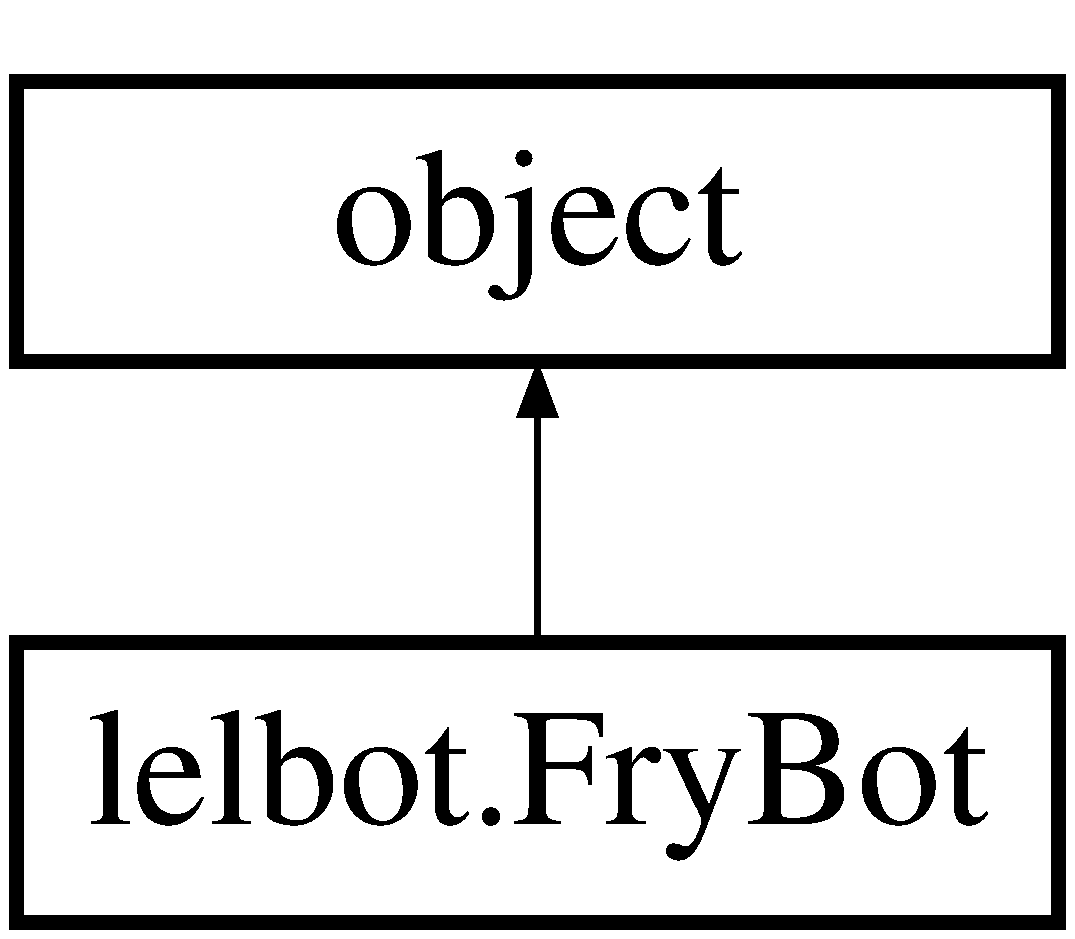
\includegraphics[height=2.000000cm]{classlelbot_1_1_fry_bot}
\end{center}
\end{figure}


The documentation for this class was generated from the following file\+:\begin{DoxyCompactItemize}
\item 
C\+:/\+Users/auntfox/\+Desktop/frybot\+\_\+test2/lelbot.\+py\end{DoxyCompactItemize}

%--- End generated contents ---

% Index
\backmatter
\newpage
\phantomsection
\clearemptydoublepage
\addcontentsline{toc}{chapter}{Index}
\printindex

\end{document}
